\documentclass[11pt]{article}

\usepackage[utf8]{inputenc}
\usepackage[T1]{fontenc}
\usepackage{lmodern}
\usepackage[margin=1in]{geometry}
\usepackage{booktabs}
\usepackage{graphicx}
\usepackage{amsmath}
\usepackage{hyperref}
\usepackage{xcolor}
\hypersetup{colorlinks=true, linkcolor=black, citecolor=black, urlcolor=blue}

\newcommand{\dmodel}{\ensuremath{d_{\text{model}}}}
\newcommand{\code}[1]{\texttt{#1}}

\title{When does learned root-cause attribution beat a one-line heuristic?}
\author{Samarth Kulshrestha\\ \small\texttt{samarth.kulshrestha@lyriem.com}}
\date{}

\begin{document}
\maketitle

\begin{abstract}
We tried to learn root-cause attribution over program execution traces with an attention model, and we report a negative result. On use-after-free, the one bug class with an automatic sanitizer oracle, the cause is by definition the most-recent same-object event before the crash, so a one-line heuristic attributes it perfectly (Hit@1 $= 1.000$) and the learned model does not. We then built synthetic benchmarks where recency fails by construction. There a cause-supervised model recovers the planted relational signal, reaching Hit@1 around $0.88$ against a recency baseline near zero, but it never beats the generator's own oracle rule, and it ties or loses to a plain bidirectional LSTM. Ablating the bidirectional attention we designed the system around shows the mechanism does not help; on the real corpus it hurts, where a backward-only model scores $0.976$ against the bidirectional model's $0.824$. On one real bug from the mjs interpreter our pipeline maps the sanitizer report onto the trace, but that trace contains a single free, so attribution is not measurable and one example is not a training set. The regime where learning might help, a distal cause among several plausible frees, is the same regime that has no automatic oracle, which we could not label at scale. We give the boundary and the reasons for it.
\end{abstract}

\section{Introduction}

Debugging tools find the symptom of a failure: the line that crashed, the event a detector flags as anomalous. The harder problem is attribution, which points back through the execution to the earlier event that caused the symptom. A use-after-free crashes at the use, but the fault is the earlier free. The appealing idea is that an attention model trained over traces would learn to connect the two, and that the attention weights would then read out as an explanation. We built that system from scratch and set out to test the claim. The claim did not hold, and the shape of the failure is what we report.

We found four things, in the order we found them. On use-after-free, labeled automatically by AddressSanitizer, the cause is the most-recent same-object event before the crash, so a one-line heuristic gets a perfect score and the learned model trails it. On a synthetic benchmark built so that recency fails, the generator's own oracle rule is again perfect and the model is not. A plain bidirectional LSTM matches or beats our attention architecture on that same benchmark. And on a real bug the pipeline reaches, the heuristic still wins and the model cannot be trained at all. Figure~\ref{fig:summary} collects the numbers. The learned model wins no benchmark. We publish that boundary rather than search for a framing in which it looks like a win.

\begin{figure}[t]
  \centering
  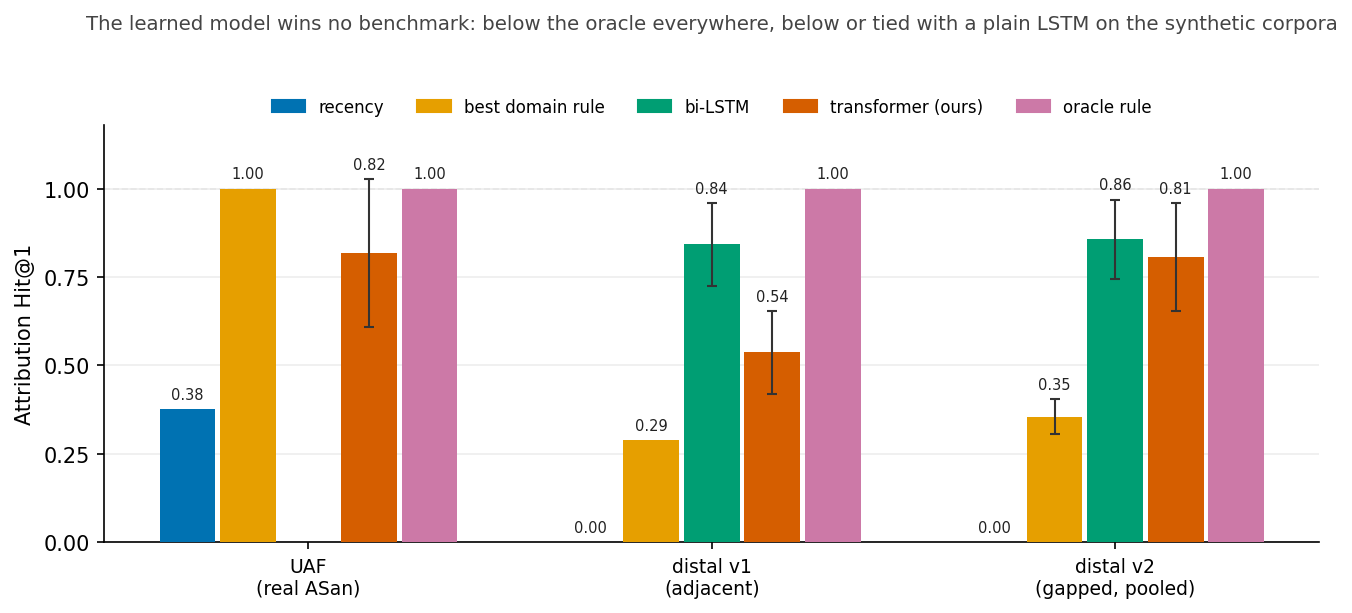
\includegraphics[width=\linewidth]{fig1_summary.png}
  \caption{Attribution Hit@1 by corpus and method. The learned transformer sits below the oracle rule on every corpus and at or below a generic bi-LSTM. It clears only the raw-recency baseline. Error bars are $\pm$ standard deviation over seeds; deterministic rules have none. Produced by \code{fig1\_summary.py}.}
  \label{fig:summary}
\end{figure}

The reason the result is worth reporting, rather than filing as a failed experiment, is that the failure has a clean structure. Learning does not help where an automatic oracle exists, because the property that creates the oracle (the cause is the most-recent related event) also solves the problem in one line. Learning might help where the cause is distal, but that regime has no automatic oracle, so there is no cheap way to get the labels a model needs. The gap between the two is not a modeling gap. It is a data-acquisition wall, and we walked into it on real code.

\section{Problem and setup}

A trace is a sequence of function-call events. Each event carries a timestamp, a set of hardware counters, and an object id derived from the allocation address captured at run time, so that events touching the same heap object share an id. Given a trace with a known crash event (the symptom), the attribution task is to rank the other events so that the true cause is near the top. We score with Hit@1, Hit@3, and mean reciprocal rank over the candidate events, excluding the crash itself.

We use three corpora. The first is a set of real executions of small templated C programs, compiled with AddressSanitizer and function instrumentation, run, and labeled from the sanitizer report; this is our use-after-free negative control. The other two are synthetic distal-cause generators, v1 (adjacent) and v2 (gapped), whose labels are injected by construction. The model is a transformer encoder written from scratch in Rust, with \dmodel${}=64$, four heads, two layers, and a window of 64 events. We do not treat the implementation as a contribution; it is the apparatus.

Two facts about the comparison are stated here because they favor the model and it loses anyway. The model is trained with supervision on the ground-truth cause (\code{attribution\_lambda = 1.0}), while every heuristic baseline is unsupervised. The LSTM baseline gets the same cause supervision. And at object bias above zero, the model is handed a same-object attention prior, which is the heuristic answer wired directly into the attention scores. A model that carries both advantages and still loses to an unsupervised one-liner is losing on the merits.

\section{Use-after-free: the negative control}

For a use-after-free, the cause is the most-recent same-object event before the crash. This holds by definition, not by measurement: once an object is freed, nothing valid touches it again, so the free is the last same-object access before the invalid use. A heuristic that ranks the most-recent same-object event first therefore attributes every use-after-free correctly. On our real sanitizer-labeled corpus it scores Hit@1 $= 1.000$.

The supervised model does not match this. With no object bias it scores $0.488 \pm 0.145$. It rises to $0.824 \pm 0.247$ and $0.893 \pm 0.125$ only as we increase the injected same-object prior to bias 4 and bias 8. That prior is the heuristic wired into attention, so the higher numbers are an oracle upper bound and not a learned ability. Plain positional recency, with no object information, scores $0.378$. Spectrum fault localization scores $0.000$, because every function in this corpus appears in both passing and failing runs, which leaves coverage statistics with no signal.

These numbers survive two checks. Pooled over three independent corpus realizations, the bias-4 model holds at $0.818 \pm 0.210$, so the result is not an artifact of one generated corpus. And under a crash-window evaluation that scores the window containing the crash rather than the first window of the trace, no traces are dropped, because the templated programs are short enough that the crash always falls in the first window. Use-after-free is a clean negative control: it is the bug class with a free oracle, and it is exactly the class where learning is unnecessary.

\section{Distal causes: a capability probe}

If learning can help anywhere, it should be where the cause is distal, not the most-recent related event, so that recency fails. We built a generator for that regime. The final version, v2 (gapped), places a \code{trigger} marker carrying the real object id, then inserts a verified gap of at least two same-object events before the causal write, so that no adjacency rule can recover the cause and no baseline is blind to the marker. The label is the first same-object write after the same-object trigger.

Table~\ref{tab:ladder} gives the full ladder on v2 at object bias 4.

\begin{table}[t]
  \centering
  \caption{Attribution on the v2 (gapped) distal corpus, single corpus realization, bias 4. Mean $\pm$ standard deviation over five model seeds; deterministic rules have zero variance.}
  \label{tab:ladder}
  \begin{tabular}{lccc}
    \toprule
    rule or model & Hit@1 & Hit@3 & MRR \\
    \midrule
    recency & $0.000 \pm 0.000$ & $0.000 \pm 0.000$ & $0.113 \pm 0.000$ \\
    same-object recency & $0.000 \pm 0.000$ & $0.538 \pm 0.000$ & $0.295 \pm 0.000$ \\
    same-object write & $0.333 \pm 0.000$ & $1.000 \pm 0.000$ & $0.658 \pm 0.000$ \\
    Ochiai FL & $0.000 \pm 0.000$ & $0.000 \pm 0.000$ & $0.113 \pm 0.000$ \\
    Tarantula FL & $0.000 \pm 0.000$ & $0.000 \pm 0.000$ & $0.113 \pm 0.000$ \\
    trig-adjacent (v1 oracle, now dead) & $0.026 \pm 0.000$ & $0.026 \pm 0.000$ & $0.137 \pm 0.000$ \\
    trig-window (oracle) & $\mathbf{1.000 \pm 0.000}$ & $1.000 \pm 0.000$ & $1.000 \pm 0.000$ \\
    bi-LSTM (supervised) & $0.856 \pm 0.113$ & $0.964 \pm 0.038$ & $0.913 \pm 0.068$ \\
    transformer (supervised, bias 4) & $0.877 \pm 0.068$ & $0.985 \pm 0.031$ & $0.929 \pm 0.044$ \\
    \bottomrule
  \end{tabular}
\end{table}

Three things follow from the table. First, rule-labeled synthetic data always has a perfect oracle rule, because the label is a rule; here it is \code{trig-window} at $1.000$, and a strictly simpler rule (``the second same-object write, in order'') also solves it. We say this plainly so the benchmark is read as a capability probe and not as evidence that the model beats hand-written rules. It does not. Second, the transformer and the LSTM tie. The transformer scores $0.877 \pm 0.068$ on a single corpus and $0.807 \pm 0.152$ pooled over three; the LSTM scores $0.856 \pm 0.113$. The transformer carries the injected object prior and the LSTM does not, so a tie is evidence that the attention architecture adds nothing over a generic sequence model. Third, data-seed variance matters: the deterministic oracle stays at $1.000 \pm 0.000$, but the same-object-write baseline moves to $0.355 \pm 0.050$ once we vary the corpus, which shows the $\pm 0.000$ we first reported for non-oracle baselines was one draw and not stability.

What survives is narrow. Cause supervision recovers the planted relational signal, well above recency and above spectrum fault localization. It does not clear the oracle rule, and it does not clear the LSTM.

\subsection{A retracted benchmark}

Our first generator, v1 (adjacent), emitted the \code{trigger} and the causal write as one atomic step, so the cause was always the event right after a trigger, and the trigger carried object id 0, which made it invisible to the same-object baselines we compared against. We first read this as the model ($0.537 \pm 0.118$) beating the best hand-coded rule (same-object write, $0.289$). That reading was wrong. The adjacency rule \code{trig-adjacent} scores $1.000 \pm 0.000$ and we had simply not implemented it. On v1 the LSTM ($0.842 \pm 0.117$) also beats the transformer outright. We keep v1 in the record as an example of how a self-constructed benchmark manufactures a positive result, and as the reason we now implement the strongest hand rule before claiming a model beats hand rules.

\section{Ablations}

\paragraph{Bidirectional versus causal attention.}
The system is built around bidirectional attention, on the argument that a cause can precede or follow its symptom in a trace. We had never tested it. Across three corpora, no benchmark shows bidirectionality helping, and the real corpus shows it hurting. On real use-after-free the backward-only model scores $0.976 \pm 0.031$ against the bidirectional model's $0.824 \pm 0.247$, close to the oracle and far tighter. On v1 the causal model is higher on the mean ($0.805 \pm 0.235$ versus $0.537 \pm 0.118$); on v2 the two overlap. Every cause in these benchmarks precedes its symptom, so backward-only attention is sufficient and the forward half adds noise. We dropped ``bidirectional'' from the title on this result. The forward-cause case that motivated the design appears in none of our benchmarks and remains untested.

\paragraph{Object bias.}
The object-bias prior is the same-object heuristic added to the attention scores. Table~\ref{tab:bias} sweeps it.

\begin{table}[t]
  \centering
  \caption{Model Hit@1 as a function of the injected object-bias prior. Mean $\pm$ standard deviation over five seeds.}
  \label{tab:bias}
  \begin{tabular}{lcccc}
    \toprule
    corpus & bias 0 & bias 4 & bias 8 & best rule \\
    \midrule
    UAF (real) & $0.488 \pm 0.145$ & $0.824 \pm 0.247$ & $0.893 \pm 0.125$ & $1.000$ \\
    distal v1 & $0.342 \pm 0.160$ & $0.537 \pm 0.118$ & $0.463 \pm 0.209$ & $1.000$ \\
    distal v2 & $0.441 \pm 0.139$ & $0.877 \pm 0.068$ & $0.913 \pm 0.070$ & $1.000$ \\
    \bottomrule
  \end{tabular}
\end{table}

The prior adds between $0.34$ and $0.47$ to Hit@1 where it lines up with the label structure. On v1 it stops adding value (bias 8 at $0.463 \pm 0.209$ versus bias 4 at $0.537 \pm 0.118$, overlapping), which fits the fact that v1's marker token carries no object id for the prior to key on. The model reaches the oracle rule in no cell. Much of what a reader would call ``the model's score'' is this injected prior rather than anything the model learned.

\section{A real bug}

We ran one real crash through the existing pipeline: a heap-use-after-free in the mjs JavaScript engine, triggered when an array is spliced during a \code{for-in} loop (issue \#322, CWE-416). We report it as a feasibility check on one trace, not as a measured result.

The part that works is the labeling. The pipeline maps the AddressSanitizer report onto the instrumented trace and recovers the symptom (\code{mjs\_next}, event 12211) and the cause (\code{gc\_free\_block}, event 12188) in a trace of 12{,}213 events over 178 distinct functions. The cause is genuinely distal: 23 events separate it from the crash, including a full garbage-collection sweep. This retires the concern that the sanitizer-to-event mapping would break on real code.

The part that does not work is the measurement. \code{gc\_free\_block} occurs exactly once in the trace, so a ``most-recent deallocation'' rule wins over a candidate set of size one. That is trivially correct and tells us nothing, and we do not count it as a heuristic win. Positional recency ranks the true cause 24th, which again only shows that domain-agnostic recency is the wrong rule for a distal cause. The learned model cannot be run here at all: one trace is not a training set, and the crash sits in the last of 191 windows, past the point our first-window evaluation would have looked. The case that would matter (many candidate frees, with the causal one ambiguous) does not occur in this proof of concept. Reaching it needs many labeled real traces, which is the data-acquisition wall again.

\section{Threats to validity}

\paragraph{Single-corpus variance.}
Except where we state a pooled number, each $\pm$ is over five model-init seeds on one corpus realization and one train/test split. The $\pm 0.000$ on a deterministic baseline means ``one draw,'' not ``stable,'' and would move under a different data seed, as the same-object-write row in Table~\ref{tab:ladder} does when we vary it. We report data-seed variance for use-after-free and v2; the others are single-realization. We run no significance test. The two inequalities we rely on (LSTM at or above the transformer on v1, and model below the oracle everywhere) are large or true by construction, but the smaller gaps we describe as ties.

\paragraph{Selection by window.}
The evaluation now scores the window containing the crash and reports a drop count for anomalous traces whose cause falls outside that window. On the templated corpus the drop count is zero, so its numbers are unchanged. The filter was real, though: the mjs crash sat in window 191 and the old first-window evaluation would have dropped it silently. On a longer corpus this filter would bias the retained set toward traces where the cause sits near the crash, which is where recency is trivially right.

\paragraph{Scope.}
All corpora share one program family or one generator, so cross-program generalization is unmeasured. The evaluation is at small scale (\dmodel${}=64$, two layers, window 64) with roughly 38 to 84 anomalous test traces per corpus, most of them synthetic. The interesting regime, distal causes, has no automatic oracle, so we could not build a real corpus for it; that is the central limitation and the reason the positive claim stays hypothetical.

\paragraph{Baseline fairness.}
The LSTM trains on a single objective (cause cross-entropy) while the transformer trains on several. On the synthetic corpora both models see whole traces of at most 64 events, so windowing is not a confound there. The remaining asymmetry, the transformer's extra losses and its object prior, favors the transformer, which still ties or loses.

\section{Related work}

Bidirectional encoders over log and trace sequences are established; LogBERT and DeepLog are the standard references, and our bidirectional framing is not new. Attention rollout (Abnar and Zuidema, 2020) is one way to turn attention into an attribution map; we tried it and fell back to raw last-layer, head-averaged attention. Spectrum-based fault localization (Ochiai, Tarantula) is a classic non-learned baseline. It is blind on our corpora because it ranks functions by cross-trace coverage, and here every function appears in both passing and failing traces; we include it as a floor, not a competitor.

\section{Conclusion}

The honest summary is that learned attribution earns its keep in none of the settings we could measure. Where an automatic oracle exists, the oracle also gives a one-line rule that the model cannot beat. Where the cause is distal and a model might help, we have no oracle and so no labels, and a real trace in that regime was not measurable with one example. Our bespoke attention model does not beat a plain LSTM, and its defining bidirectional mechanism does not help. The useful output of this work is the boundary itself: a clear statement of where learning cannot help because a heuristic already wins, and where it might help but the data does not yet exist. We would rather leave that marker in the ground than move it to make the model look better.

\end{document}
